\section{Results} \label{sec_results}
In this Section, we compare the solution of the problem on an uniform mesh
with the one on Z-mesh \cite{Stone2003}. We also show that the
discretization used can easily handle unstructured polygonal grid. Finally, we
conclude this section with an example of AMR mesh.
\subsection{Z-mesh}
The Z-mesh is defined as in \Cref{fig_z_mesh} where $\alpha$ is a parameter
$\in [0,0.5]$. 
\begin{figure}[H]
  \centering
  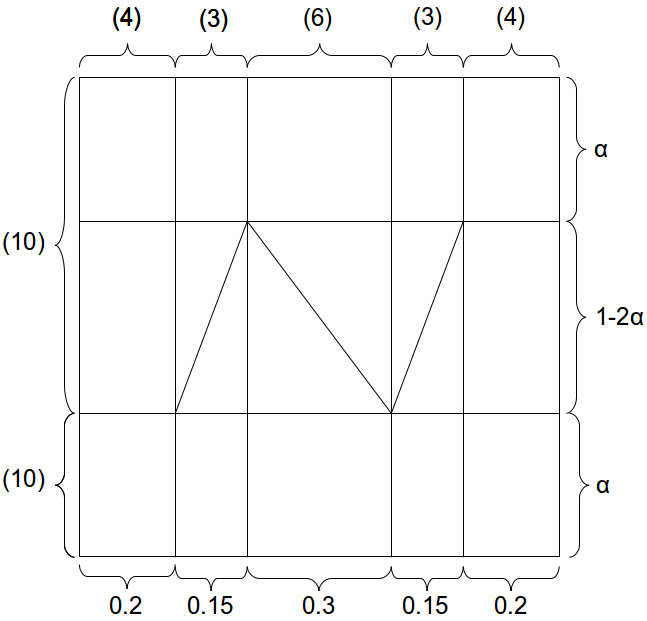
\includegraphics[width=5cm]{z_mesh}
  \caption{Z-mesh ((x) is the number of divisions and Y is the distance in cm)}
  \label{fig_z_mesh}
\end{figure}    
We compare the solution of the diffusion equation using the Z-mesh
\Cref{z_mesh_sol} with $\alpha=0.2$ with the one obtained using an uniform \Cref{u_mesh_sol}. 
The domain is 1cm by 1cm and is discretized using 20 by 20 cells. All the 
boundary conditions are vacuum. The medium is homogeneous $\Sigma_a = 0.5 cm^{-1}$ 
and $D=2$. There is a uniform source of intensity 1.                  
\begin{figure}[H]
  \centering
  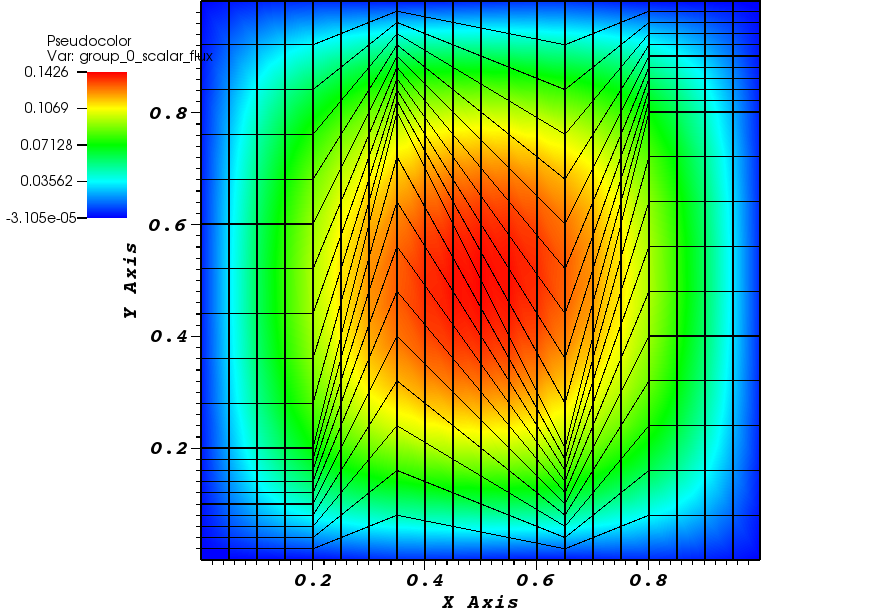
\includegraphics[width=5cm]{z_mesh_sol}
  \caption{Scalar flux on the z-mesh}
  \label{z_mesh_sol}
\end{figure}
\begin{figure}[H]
  \centering
  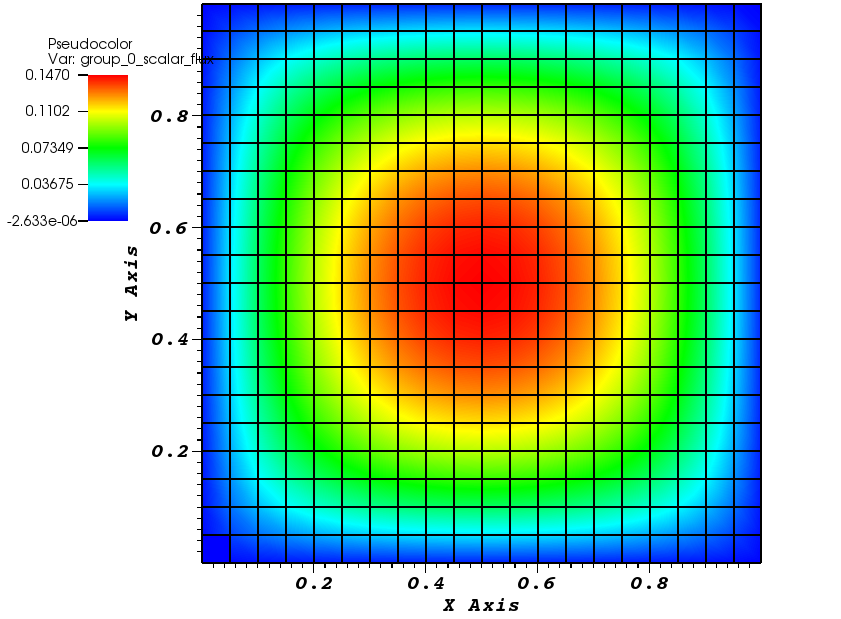
\includegraphics[width=5cm]{pwld_uniform_sol}
  \caption{Scalar flux on the uniform mesh}
  \label{u_mesh_sol}
\end{figure}
\subsection{Randomized polygonal grid}
\subsection{AMR}
